\chapter{Baseline}\label{ch:baseline}

In this chapter, we describe the baseline implementation.
We first describe the mental model
associated with this simpler version
of the protocol (\cref{sc:baseline-mental-model}).
Then, we detail the motivation for this work (\cref{sc:baseline-motivations}).
We end this chapter with a description of the
implementation, providing the details
that are more relevant (\cref{sc:baseline-protocol}).
We highlight that, even though we use well-established
cryptographic primitives, we found it
challenging to implement the baseline correctly
with the limited support provided by the
Web Crypto API.
The cryptographic expertise of both supervisors
of this thesis was really helpful to ensure that the
workarounds we use are secure.

\section{Mental Model}\label{sc:baseline-mental-model}
The baseline is a simple version of the SSF scheme.
As in the SSF scheme, the baseline goal is to provide users, organised in groups, with
the ability to share files among members of the group in
a secure way.
Users are identified through a PKI.
A ``shared folder'' is a collection of files that are shared 
among a group of users. 
The group membership can change.
The file content 
should be accessible only to the users participating 
in the folder. Users use E2EE to ensure the confidentiality
of file contents.
Storage space for the files is
provided by a cloud storage provider. 
Differently from the SSF scheme, advanced security guarantees
like IAC (\cref{sc:iac}) and the admin role (\cref{sc:mental-model}) are not part of the baseline.
Since admins are not part of the baseline, users can only remove themselves from a group, but they cannot remove other users from the group.
The baseline does not provide any mechanism to rotate the group key.

\section{Motivation}\label{sc:baseline-motivations}

The main motivation for the baseline implementation is
to create a simple client to test the infrastructure which 
will be used by the SSF implementation as well.
With this first client, we avoid adding the cryptographic complexity of the SSF scheme, and we can focus
on the server components and client-server communication.

A secondary future use of the baseline is to provide a
na\"ive implementation of a file sharing system 
for performance comparison with the SSF implementation (\cref{sc:future-work}). 

\section{Cryptographic Protocol and Key Hierarchy}\label{sc:baseline-protocol-hierarcy}

The baseline uses simple cryptographic primitives, instantiated with the following algorithms:
\begin{itemize}
    \item Symmetric encryption based on Advanced Encryption Standard Galois/Counter mode (AES-GCM) with 256-bit keys.
    \item Message authentication code, HMAC, using SHA-256 hashing algorithm. 
    \item Key derivation function, HKDF, using the SHA-256 hashing algorithm.
    \item Elliptic curve integrated encryption scheme (ECIES), a hybrid encryption scheme based on:
    \begin{itemize}
        \item Asymmetric Key Exchange based on elliptic curve Diffie Hellman (ECDH), using P-256 curve.
        \item Key encapsulation mechanism (KEM), based on the above ECDH and AES-GCM.    
    \end{itemize}
\end{itemize}

We now describe the key hierarchy used to encrypt files and their metadata:
\begin{itemize}
    \item Each file is encrypted with a randomly sampled symmetric key, called a file key.
    \item Each folder is associated with a randomly sampled symmetric key, called folder key. The folder key is shared among all group members.
    \item The file key and its metadata (name, authors, etc.), which we call collectively the file's ``private data'', are encrypted under the folder key.
\end{itemize}

The folder key sharing protocol is based on ECIES where the folder key
is encrypted under the long-term public key of each group member,
extracted from the user's certificate that can be fetched
from the PKI server (\cref{sc:PKI}).
The key material and file metadata encrypted as described above is
then stored in a metadata file inside the shared folder in the cloud.
The file structure is given by the \texttt{Metadata} TS interface
detailing the following content:
\begin{itemize}
    \item \texttt{folderKeysByUser}, storing for each user the folder key encrypted through ECIES, with all required parameters to perform decryption.
    \item \texttt{fileMetadatas}, for each file id (\cref{sc:ssf-proxy-server}) store its encrypted private data, i.e. the file metadata and the file encryption key.
\end{itemize}

\begin{figure}
    \centering
    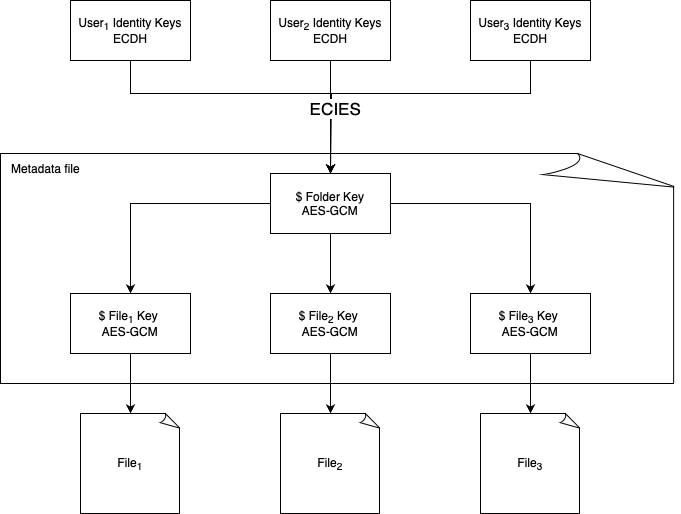
\includegraphics[width=0.8\textwidth]{figures/baseline-keys.png}
    \caption{Baseline key material: The \$ sign indicates that the key is randomly sampled. Each file is encrypted with a symmetric key, using AES-GCM. The file keys are encrypted under the folder key, through AES-GCM. The folder key is stored encrypted using ECIES for each user of the folder, under their public key signed by the PKI. 
    All the encrypted folder keys and file keys are stored in the metadata file of the folder.}
    \label{fig:baseline-protocol-hierarchy}
\end{figure}

Although the cryptographic primitives used in the baseline are
basic blocks in the cryptographic research literature,
and are standardised by the IETF, the implementation of
ECIES using the Web Crypto API (\cref{sc:webcrypto-api}) was challenging.
We document the issues and the workarounds in \cref{sc:implement-ecies}.

\subsection{Implement ECIES with the Web Crypto API}\label{sc:implement-ecies}

ECIES is not provided as a building block out-of-the-box by the Web Crypto API.
To implement ECIES, we need to first implement 
the KDF and KEM on top of the ECDH, AES-GCM and HKDF algorithms provided
by the Web Crypto API.

The file \texttt{ssf-client/protocol/kemKdf.ts} contains the code for both the KDF and KEM.
The difficulties are rooted in the fact that
in the Web Crypto API, the \texttt{CryptoKey}
object, which is an abstraction used in the API on the byte array containing the key material,
is always designated to perform a specific algorithm and
a limited set of operations.
Trying to use a \texttt{CryptoKey} object for a different algorithm or operation
will result in an error.

Specifically, the library does not allow performing 
HKDF to obtain a new HKDF designated key.
Therefore, instead of separating the implementation
of the KEM and KDF, we implemented them in one single pass.
During the derivation of the symmetric key,
We concatenate all the labels that are used, both
during the KDF and the KEM. This is not optimal,
as we cannot re-use the KDF or the KEM operations
separately, but with this workaround we do not need
to rely on more complicated techniques 
to bypass the limitations of the Web Crypto API,
as done in \cref{sc:ssf-sskg}.

We remind the reader that the KEM and KDF are used to
implement ECIES, which ultimately is used to
share the folder key with new group members.

\section{Implementation Details}\label{sc:baseline-protocol}

The file \texttt{ssf-client/protocol/baseline.ts} collects all the code specific to the baseline.
Unit and integration tests for the baseline are in the subfolder \texttt{test}.
All cryptographic modules that can be found in
\texttt{ssf-client/protocol} apart from ECIES are re-used in the SSF scheme,
and unit tests with 100\% code coverage are included in the
\texttt{test} subfolder.

\subsection{Metadata Synchronization}\label{sc:metadata-synchronization}

As mentioned in \cref{sc:ssf-proxy-server}, the
SSF Proxy server provides concurrency control
when updating the files in the cloud storage (\cref{sc:ssf-file-changes-sync}).
Since the key material is all stored encrypted in a special metadata file
in the cloud
the server needs to synchronize the metadata file updates
to ensure a consistent and ordered cryptographic state of the folder,
i.e., when two or more update requests targeting the same version of the metadata file are received, only one is
accepted, and the others are rejected, so that the
clients fetch the updated state before proceeding
with the changes, and no modifications would be lost.

The server exposes an endpoint to upload a new file
to the cloud storage. The request contains the file
content to upload, which is sent encrypted by the client
(\cref{sc:baseline-protocol-hierarcy}). The client
also needs to provide:
\begin{itemize}
    \item The ETag (version) of the metadata file on which the update is based.
    \item The new metadata content to be stored in the shared folder metadata location.
\end{itemize}
Requests where the ETag does not match the current version
of the metadata file are rejected. Given the
synchronization mechanism described in \cref{sc:ssf-file-changes-sync},
all clients will operate on consistent data, and
will not lose updates.

The first creation of the metadata file instead happens
at shared folder creation, where the server will
accept the first metadata file content upload
without requiring any ETag. A baseline client
creating a shared folder will initialise the metadata
file with the folder key encrypted under its own
public key.

The synchronization mechanism implemented
for the baseline will be re-used in the SSF scheme
implementation, see \cref{sc:ssf-file-encryption}.
